\documentclass{article}
\usepackage[utf8]{inputenc}
\usepackage{polski}
\usepackage[polish]{babel}
\usepackage{graphicx}
\begin{document}
\title{POP - projekt - sprawozdanie przedkońcowe}
\author{Adam Czupryński \and Szymon Makuch}
\maketitle

\section{Temat}
Ewolucja różnicowa z modyfikacją wdrażającą (nieszablonowy) model zastępczy (surrogate model) w celu wyboru osobników z populacji do określenia ich jakości za pomocą funkcji celu.


\section{Stan zaawansowania projektu}
\subsection{Zrealizowane cele}
Do tej pory udało nam się zaimplementować algorytm ewolucji różnicowej oraz jego drugą (zmodyfikowaną) wersję, która pozwala na użycie modelu zastępczego. W celu uzyskania większej kontroli nad algorytmem ewolucji różnicowej zdecydowaliśmy się zaimplementować go samodzielnie zamiast używać zewnętrznej biblioteki. 
W ramach modelu zastępczego planujemy zaimplementować algorytm ID3, jednak na ten moment kożystamy z gotowej klasy "DecisionTreeRegressor" z biblioteki scikit-learn.
Ponadto stworzyliśmy testy jednostkowe oraz podstawowe wykresy sprawdzające czy nasz algorytm działa poprawnie.

\subsection{Wykresy przedstawiające działanie algorytmu}
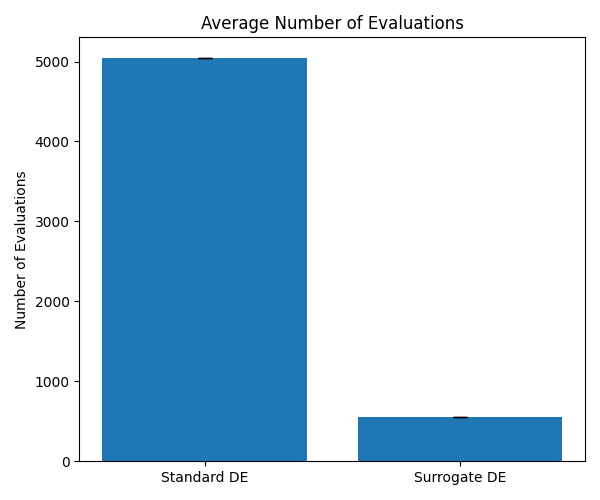
\includegraphics[scale=0.7]{results_evaluations.png}

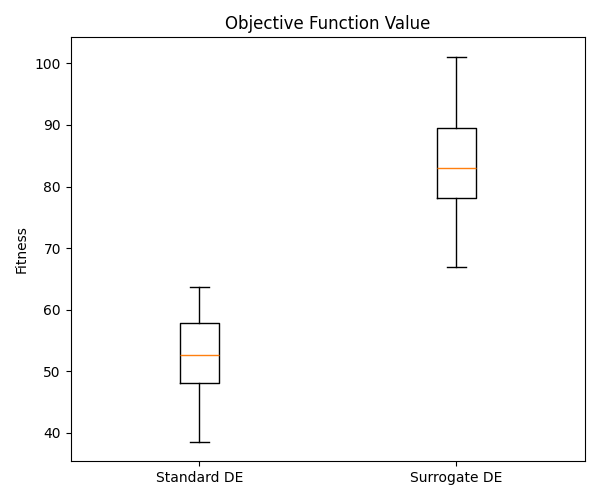
\includegraphics[scale=0.7]{results_fitness.png}

\subsection{Pozostałe cele}
\begin{itemize}
   \item Przeprowadzenie eksperymentów porównawczych
   \item Implementacja większej liczby funkcji testowych (w tym z benchmarku CEC)
   \item Implementacja algorytmu ID3
   \item Dokładna analiza wyników
\end{itemize}


\end{document}